\documentclass[11pt,dvipdfmx,b5paper]{jsbook}
%\documentclass[11pt,dvipdfmx,a5paper,oneside]{jsbook}

% -------------
% 基本パッケージ
% -------------
\usepackage{graphicx}
\usepackage{booktabs}
\usepackage{caption} % 図表のキャプションを変更する
\usepackage{geometry} % ページレイアウトを変更する
\usepackage{here} % 画像を強制的にその場に表示させる
\usepackage{framed} % 改ページ可能なフレームの生成
\usepackage{wrapfig} % 図の周りにテキストを回り込ませる
\usepackage{algorithm} % 疑似コードを書くためのパッケージ
\usepackage{listings} % ソースコードを書くためのパッケージ
%\usepackage{balance} % 2カラム文書を書く場合に左右カラムでバランスを取る

% -------------
% フォント系パッケージ
% -------------
\usepackage[utf8]{inputenc} % 文字コードを指定
\usepackage{microtype}
\usepackage[T1]{fontenc} % フォントのエンコーディングを指定
\usepackage{lmodern} % ラテンモダンフォントを指定
\usepackage{xcolor} % 文字の色を変えられるように

% -------------
% 数学表記系パッケージ
% -------------
\usepackage{latexsym} % 数式で使える記号を増やす
\usepackage{amsmath} % 数式を書くためのパッケージ
\usepackage{bm} % 太字のベクトルを書けるように

% -------------
% リンク/目次系パッケージ
% -------------
\usepackage{url} % URLを書けるように
\usepackage[hidelinks]{hyperref} % ハイパーリンク付き文書を書けるように
\usepackage{pxjahyper} % hyperrefの機能を拡張する

% -------------
% 装飾系パッケージ
% -------------
%\usepackage{quotchap} % 章見出しを装飾する
%\usepackage{titlesec} 見出しの書式を変える
\usepackage[most]{tcolorbox} % 枠囲みを作成するパッケージ
%\usepackage{tikz} % tcolorboxとセットで使う

% -------------
% 執筆補助パッケージ
% -------------
\usepackage{lineno} % 行番号を表示
%\linenumbers

% -----------------
% 自作の関数・スタイル
% -----------------
% -------------
% 文字数・行数設定
% -------------
% 1行あたりの文字数
\setlength { \textwidth } { 37zw }
% 1ページあたりの行数
\setlength { \textheight } { 32\baselineskip }

% -------------
% 自作カラー
% -------------
\definecolor{brandblue}{rgb}{0.34, 0.7, 1}
\definecolor{background}{rgb}{0.94,0.95,0.96}
\definecolor{turquoisegreen}{rgb}{0.63, 0.84, 0.71}

% -------------
% 自作修飾
% -------------
%\newcommand{\red}[1]{\textcolor{red}{#1}}
\newcommand{\graybox}[1]{\colorbox[gray]{0.9}{\texttt{#1}}}
\newcommand{\strong}[1]{\textbf{#1}}

% -------------
% 自作スタイル
% -------------
\tcbset {
  base/.style={
    arc=0mm,
    bottomtitle=0.5mm,
    boxrule=0mm,
    %colbacktitle=black!10!white,
    coltitle=black,
    fonttitle=\bfseries,
    %leftrule=1mm,
    %left=2.5mm,
    left=3.5mm,
    right=3.5mm,
    title={#1},
    toptitle=0.75mm,
  }
}

\newtcolorbox{mainbox}[1]{
  colframe=brandblue,
  base={#1}
}

\newtcolorbox{notebox}[1]{
  colframe=brandblue,
  base={Note - #1}
}

\newtcolorbox{warningbox}[1]{
  colframe=orange,
  base={注意 - #1}
}

\newtcolorbox{tipbox}[1]{
  colframe=turquoisegreen,
  base={Tip - #1}
}

\newtcolorbox{subbox}[1]{
  colframe=black!30!white,
  base={#1}
}

\usepackage{minted}
\usemintedstyle[sql]{tango}


% ------------
% コンテンツ
% ------------
\begin{document}

\chapter{データベースを使わない世界}

データベースと聞いて何を思い浮かべるだろうか.
大抵の人は,データベースといえば「大きなデータの集まり」といったイメージを持つのではないだろうか.
このイメージはあながち間違いではない.

さて,本講義のようにわざわざ科目を立ててまで,データベースについて学ぶことはあるのだろうか?
結論としては,大規模データに携わるITエンジニアやデータ分析者を目指す人であれば,「大いにあり」である.
1960年代から今日に至るまで,データベース技術は盛んに研究開発が行われてきた.
大きなデータの集まりを扱うには,対処しなければならない問題が思った以上に数多く存在するのである.

本講義では10数回にわたってデータベース技術について解説するが,この第1講ではデータベースのことはいったん横に置いておいておく.
今回は(割と)大きなデータを扱うときに遭遇する問題について考えてみよう.


\section{ケース1: 販売履歴の記録をはじめる}
以下は,山畑さんという架空の人物のお話である.

\begin{framed}
山畑さんは家族で小さな小売店を営んでいる.
個人経営ながら山畑さんのお店は繁盛している.
とはいえ,街には大手チェーン小売店が進出してきており,このまま順調に経営を続けられるか,不安が募っている.
何か手を打たなければならない.

2020年の4月,山畑さんは念願のショッピングサイトを立ち上げた.
言うまでもない.
ショッピングサイトを立ち上げたのは,オンラインの場にも顧客獲得の機会を求めるためだ.
サイトは順調に立ち上がり,注文もポツポツ入ってきている.

ところで,最近「データサイエンス」なるものが世間の注目を集めているらしい.
データを活かせばビジネスチャンスが広がるとのことだ.
山畑さんは,Excelシートに記録を取り始めた販売履歴を分析してみようと思い立った.

山畑さんが使っているExcelシートには,「いつ,誰が,何を,いくらで購入したか」の情報が記録されている.
ショッピングサイトは立ち上がったばかりであり,Excelシートには200行しかデータが入っていない.
しかし,今後データが貯まっていけば,売り上げを増やすための課題が見えるかもしれない.
いずれがっつりとデータ分析をやるためにも,山畑さんは手持ちのデータを用いて分析の練習に取り組むことにした.
\end{framed}


\subsection*{データの確認}
こちらのURL(\url{https://dbnote.hontolab.org/data/purchase\_small.xlsx})から,上のケース1で山畑さんがデータ分析の練習に使おうとしているExcelファイル(\graybox{purchase\_small.xlsx})をダウンロードし,中身を確認しなさい.

なお,Excelシートの各列の意味は以下の通り:
\begin{itemize}
\item purchased\_at: 購買(販売)日時
\item customer: 商品を購入した人物の氏名
\item gender: 商品を購入した人物の性別
\item product: 購入された商品名
\item sale: 販売価格
\end{itemize}


\subsection*{あの人は何回買い物をしている?}
「岡田 真綾」という人物が何回買い物をしていたかを数えなさい.


\subsection*{商品Xを購入しているのは誰?}
Excelのオートフィルタ機能を使って,「ビタミン補助剤」を購入している人をリストアップしなさい.


\subsection*{総売上金額}
Excel関数の\graybox{\texttt{SUM}}を用いて,現時点での総売上金額を計算しなさい.


\subsection*{最も売れた商品は?}
Excelのピボットテーブル機能を使って,集計期間中に
\begin{itemize}
\item 最も購買回数が多かった商品
\item 最も売上金額の合計が大きかった商品
\end{itemize}
をそれぞれ求めなさい.



\section{ケース2: サイトの認知度向上につき,得られるデータも膨大に!?}
現時点では手持ちのデータは少ないものの,販売履歴データの分析に将来性を感じた山畑さん.
販売履歴データを有効活用できるよう,ショッピングサイト運営により力を入れる決意を固めたのであった.

以下は,山畑さんのその後の話(架空の話)である.

\begin{framed}
ショッピングサイト立ち上げ以降,順調に利用者数も増えていった.
やはりメディアに取り上げられたのが大きかったのだろう.
あのタイミングでサイトの認知度が一気に高まり,サイトの利用者数や利用頻度も加速度的に増えていった.
それに伴い,サイト運営に関わるスタッフも増員した.

販売履歴の管理は,当初は山畑さんが一人で担当していたが,さすがに一人では対応しきれなくなった.
そこで,ある時点から数名体制で販売履歴の記録を行うことになった.
これまで販売履歴の管理に使ってきたExcelシートをクラウドストレージに置き,記録担当スタッフのPC間で同期を取る仕組みを導入.
同じExcelファイルの上で,スタッフ全員で販売履歴を記録できるようにしたのである.

2年後.サイト事業は軌道に乗った.
十分な量の販売履歴データが蓄積されたと判断した山畑さんは,いよいよ大規模な販売履歴データの分析に取りかかることを決意した.
立ち上げ当初は200〜300行しかなかったExcelシートであったが,シートを開きその行数を数えてみると…
なんとその数90万行以上!
データの量に小躍りした山畑さんは,Excelシートの扱いに詳しいスタッフと共に,意気揚々とデータ分析に取りかかったのであった.
\end{framed}


\subsection*{データの再確認}
こちらのURL(\url{https://dbnote.hontolab.org/data/purchase\_large.xlsx})から,上のケース2で山畑さんが分析しようとしているExcelファイル\graybox{purchase\_large.xlsx}をダウンロードしなさい.
またダウンロードしたファイルを用いて下記課題(演習1と同じ)に取り組み,データ分析上の課題(困ったこと)を議論しなさい.
以下,課題1の内容を再掲する.
\begin{itemize}
    \item 「岡田 真綾」という人物が何回買い物をしていたかを数えよ
    \item 「ビタミン補助剤」を購入している人をリストアップせよ
    \item 総売上金額を計算せよ
    \item 集計期間中に「最も購買回数が多かった商品」「最も売上金額の合計が大きかった商品」を求めよ
    \end{itemize}
もし,\graybox{purchase\_large.xlsx}ファイルがうまく開けない場合は,こちらのURL(\url{https://dbnote.hontolab.org/data/purchase\_medium.xlsx})からダウンロードできる\graybox{purchase\_medium.xlsx}を用いなさい.
なお,ダウンロードできるExcelシートの構造はケース1で用いた\graybox{purchase\_small.xlsx}と同じである.


\section{おわりに}
ケース1および2で用いたExcelファイルは,販売履歴データの集まりであった.
一般的な認識からすると,このようなデータの集まりは「データベース」ということになるだろう.

ところで,上記演習,とりわけケース2に取り組んでみてイライラしなかっただろうか?
数万件,数十万件ある表データをExcelで扱おうとすると,さまざまな不都合が生じる(図\ref{fig:excel-disaster}).
これは,本来Excelは個人用の表計算アプリケーションであって,大規模データの管理や処理を前提として設計されていないためである.

\begin{figure}[tb]
    \centering
    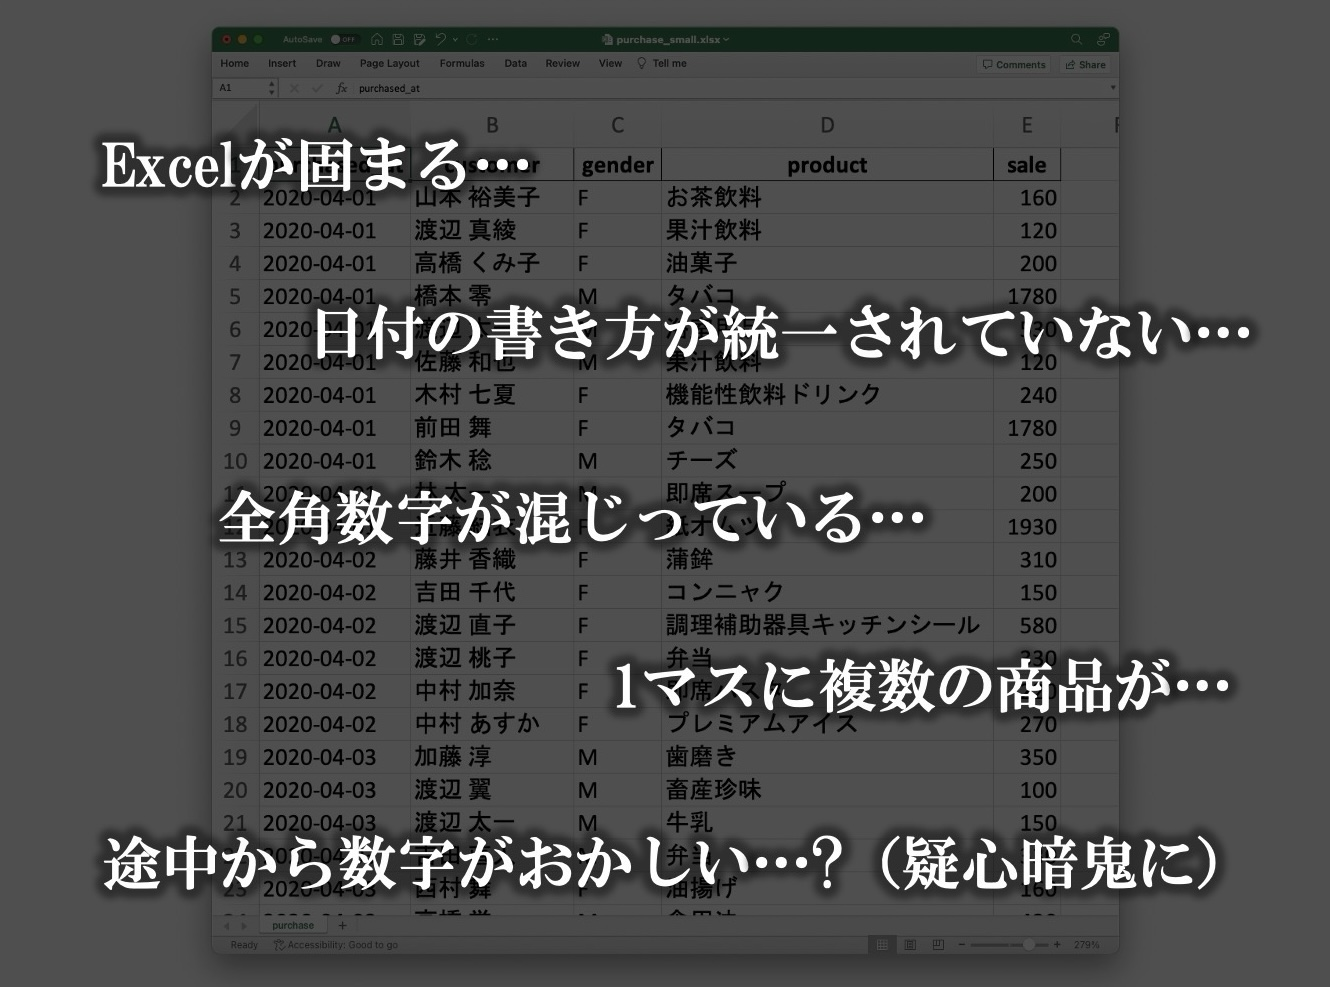
\includegraphics[width=0.8\textwidth]{figure/excel-disaster.jpg}
    \caption{大きな表データを複数人でExcelで扱うときの悲劇.}
    \label{fig:excel-disaster}
\end{figure}

では,大規模なデータを管理・処理するためにはどうすればよいだろうか?
そのための技術こそが「データベース」である.
以降,本書では\strong{大規模データを効率よく管理・処理するための「データベース」技術} について学習する.


%\chapter{SQL}
データベースからデータを引っ張ってくるなど,データベースを操作するには具体的なツールが必要となる.
\strong{SQL(Structured Query Language)} は関係データベースの操作に特化した言語である.
SQLはISOによって国際的に標準化されている.
よく用いられる関係データベース管理システム(RDBMS)としてMySQL\footnote{\url{https://ja.wikipedia.org/wiki/MySQL}}やPostregreSQL\footnote{\url{https://ja.wikipedia.org/wiki/PostgreSQL}},Oracle Database\footnote{\url{https://ja.wikipedia.org/wiki/Oracle_Database}},Microsoft SQL Server\footnote{\url{https://ja.wikipedia.org/wiki/Microsoft\_SQL\_Server}}などが挙げられるが,どのRDBMSにもSQLは実装されている.

SQLを使うことで,関係データベースのユーザは
\begin{itemize}
\item データの登録(Create)
\item データの読み出し(Read)
\item データの更新(Update)
\item データの削除(Delete)
\end{itemize}

が可能となる\footnote{データの作成,読み出し,更新,削除はデータベースに求められる主要な操作で,それぞれの頭文字を取ってCRUD(クラッド)と呼ばれる.}
なお,本教材のターゲットはデータ分析人材の卵であることから,本教材では関係データベースから\strong{データの読み出し}に焦点を当ててSQLの説明を行う.

SQLはデータベースに対する問い合わせ言語であって,プログラミング言語ではない.
そのため,プログラミング言語に比べて覚えることは少なく,問い合わせ内容を英語に近い形で書き下すことができるよう設計されている.
データ分析人材はソフトウェアを開発することが目的ではないから,高度なプログラミング能力を持つ必要は必ずしもない.
しかし,関係データベースに納められた大量のデータを自由自在に扱うためにも,\strong{SQLの習得は必須}である.


\begin{notebox}{SQLの読み方}
SQLは「エス・キュー・エル」と読む.SQLは1970年代にIBM社が開発したデータベース管理システムSystem Rの操作言語SEQUELを起源としている.関係データベースに熱狂していた世代の人の中には,SEQUELの名残でSQLのことを「シークエル」と呼ぶ人もいる.
\end{notebox}

\begin{warningbox}{SQLにも方言がある}
RDBMSによって,SQLで使用できる関数が異なったりすることがある.特にSQLiteについては,簡易的なRDMBSということもあり,他のRDBMSでは実装されている機能や関数が実装されていない場合がある.自分が書いたSQL文がうまく動作しない場合は,マニュアルに当たってみよう.
\end{warningbox}


\section{SQLと関係データモデルの比較}
SQLは関係データベースを操作する言語であり,それが扱うデータモデルは関係データモデルを実用的に拡張したものである.
「実用」のSQLデータモデルと「理論」の関係データモデルでは,同様の概念が異なる用語で定義されている.
以下,SQLと関係データモデルの用語の比較である.

\begin{table}[tb]
    \centering
    \caption{SQLと関係データモデルの用語の比較}
    \begin{tabular}{ll}
    \toprule
    \textbf{関係データモデル}             & \textbf{SQL}            \\ \midrule
    関係(リレーション; relation) & 表(テーブル; table) \\
    タプル(tuple)           & レコード or 行(row) \\
    属性(attribute)        & 列(カラム; column) \\
    定義域(ドメイン; domain)    & データ型           \\ \bottomrule
    \end{tabular}
    \end{table}

また,関係データモデルでは各属性はドメインで定義された値をもつが,
現実的にはある属性の値が存在しない,あるいは未定義(不明)のケースがありえる.
そのような状況では,特殊な値である\strong{NULL値}(ヌルと読む)を用いる.


\section{基本形}
関係データベースに対する最も典型的な問い合わせ要求は,
\begin{itemize}
\item 特定の\strong{表(table,テーブル)}から
\item \strong{列(column,カラム)} が特定の条件を満たす\strong{行(row)}\footnote{レコード(record)と呼ぶこともある.} を見つけ出し
\item 結果を表形式で出力する
\end{itemize}
ことである.
問い合わせのために記述するSQL文のことを\strong{クエリ(query)} と呼ぶ.

SQLによる代表的なクエリは,コード\ref{code:first-sql}に記したようなの形式の\strong{SELECT文}である.
\begin{figure}[tb]
    \begin{minted}[gobble=1,
        bgcolor=background,
        fontsize=\small,
        linenos=false,
        xleftmargin=0em]{sql}

    SELECT
        都道府県名
    FROM
        都道府県
    WHERE
        人口 >= 5000000;
    \end{minted}
    \captionsetup{name=コード}
    \caption{単純なSELECT文}
    \label{code:first-sql}
\end{figure}
上記クエリは,
\begin{framed}
「都道府県」テーブルから「人口」という列の値が500万以上である行を見つけ,その行の列「都道府県名」を出力してください
\end{framed}
という問い合わせ要求を表現したものである.
これら要求を表現するために,コード\ref{code:first-sql}のクエリでは
\begin{itemize}
\item \textsc{SELECT}句を用いて「問い合わせ結果に表示したい列情報」,
\item \textsc{FROM}句を用いて「参照したい表」,
\item \textsc{WHERE}句を用いて「表示する際の条件」
\end{itemize}
を指定している.
上記要求を英語に直してみると,SQL文は問い合わせ要求をできるだけ直感的に表現しようとしていることがお分かりいただけると思う.

コード\ref{code:first-sql}のクエリは単純な例ではあるが,関係データベースからデータを引っ張ってくる問い合わせについては,すべからくコード\ref{code:sql-structure}のような\textsc{SELECT}句から始まるクエリが用いられる.
\begin{figure}[tb]
    \begin{minted}[gobble=1,
        bgcolor=background,
        fontsize=\small,
        linenos=false,
        xleftmargin=0em]{sql}

    SELECT
        列名1, 列名2, ...
    FROM
        参照する表1, 表2, ...
    [WHERE 条件]
    [GROUP BY 列名1, 列名2, ...]
    [HAVING 条件]
    [ORDER BY 列名1, 列名2, ...]
    [LIMIT 数字];
    \end{minted}
    \captionsetup{name=コード}
    \caption{SQLの構文}
    \label{code:sql-structure}
\end{figure}
このうち,問い合わせ結果に表示したい情報を指定するSELECT句,および問い合わせの際に参照するテーブルを指定しているFROM句は必須である.
[ ]で囲まれた箇所については,書かなくてもSQLとして動作する.
なお,SELECTやFROM,WHERE,GROUP BY,HAVING,ORDER BY,LIMITといった句の意味のついては後ほど説明するが,各句は\strong{この順序で使う}必要がある.
例えば,HAVING句はWHERE句の後ろに書かない.
また,クエリの末尾にはピリオド(;)をつけ忘れてはいけない.

以後,SQLの基礎について説明する.
説明には,独立行政法人統計センターが公開している教育用標準データセット(SSDSE)の基本素材SSDSE-E\footnote{\url{https://www.nstac.go.jp/use/literacy/ssdse/\#SSDSE-E}}(データの解説はこちら)から抜粋・加工したデータ(populationテーブル)を用いる.
表\ref{tab:population-table}の通り,populationテーブルには,47ある各都道府県に関する総人口,小学校児童数,中学校生徒数,高等学校生徒数,大学学生数のデータが2021年度,2020年度分格納されている.
このテーブルが格納された関係データベースが手元にあると想定して,SQLの使い方を説明する.
\begin{table}[tb]
    \centering
    \caption{SSDSE-Eから抜粋・加工したデータ: populationテーブル}
    \scalebox{0.73}{
    \begin{tabular}{@{}rrrrrrrr@{}}
    \toprule
    \textbf{地域コード} & \textbf{都道府県} & \textbf{調査年度} & \textbf{総人口} & \textbf{小学校児童数} & \textbf{中学校生徒数} & \textbf{高等学校生徒数} & \textbf{大学学生数} \\ \midrule
    R01000 & 北海道 & 2021 & 5183000 & 231714 & 122742 & 115335 & 79729 \\
    R02000 & 青森県 & 2021 & 1221000 & 54460  & 29940  & 30543  & 15419 \\
    R03000 & 岩手県 & 2021 & 1196000 & 55597  & 30269  & 29980  & 11340 \\
    R04000 & 宮城県 & 2021 & 2290000 & 112246 & 58748  & 55329  & 49580 \\
    R05000 & 秋田県 & 2021 & 945000  & 38992  & 21924  & 21448  & 8904  \\
    &        &      &          & $\vdots$  &        &        &       \\
    % R06000 & 山形県  & 2021 & 1055000  & 49164  & 26969  & 27233  & 11801  \\
    % R07000 & 福島県  & 2021 & 1812000  & 85322  & 46148  & 45647  & 14385  \\
    % R08000 & 茨城県  & 2021 & 2852000  & 135782 & 72465  & 71842  & 30147  \\
    % R09000 & 栃木県  & 2021 & 1921000  & 95315  & 51170  & 49674  & 20496  \\
    % R10000 & 群馬県  & 2021 & 1927000  & 94185  & 50841  & 48521  & 28772  \\
    % R11000 & 埼玉県  & 2021 & 7340000  & 363199 & 187395 & 163986 & 109500 \\
    % R12000 & 千葉県  & 2021 & 6275000  & 306105 & 158265 & 141358 & 106037 \\
    % R13000 & 東京都  & 2021 & 14010000 & 622820 & 311049 & 301712 & 676964 \\
    % R14000 & 神奈川県 & 2021 & 9236000  & 451098 & 226599 & 195931 & 171164 \\
    % R15000 & 新潟県  & 2021 & 2177000  & 103680 & 53720  & 51594  & 27546  \\
    % R16000 & 富山県  & 2021 & 1025000  & 47818  & 26146  & 26068  & 10857  \\
    % R17000 & 石川県  & 2021 & 1125000  & 56620  & 30336  & 29764  & 27627  \\
    % R18000 & 福井県  & 2021 & 760000   & 39236  & 21196  & 20701  & 10065  \\
    % R19000 & 山梨県  & 2021 & 805000   & 38572  & 20955  & 22717  & 16097  \\
    % R20000 & 長野県  & 2021 & 2033000  & 101932 & 55189  & 52632  & 17032  \\
    % R21000 & 岐阜県  & 2021 & 1961000  & 101805 & 54493  & 50563  & 20185  \\
    % R22000 & 静岡県  & 2021 & 3608000  & 183614 & 98192  & 91613  & 33778  \\
    % R23000 & 愛知県  & 2021 & 7517000  & 405839 & 209151 & 185920 & 176722 \\
    % R24000 & 三重県  & 2021 & 1756000  & 90040  & 47567  & 44229  & 14062  \\
    % R25000 & 滋賀県  & 2021 & 1411000  & 80289  & 41086  & 36673  & 31242  \\
    % R26000 & 京都府  & 2021 & 2561000  & 119892 & 65187  & 66457  & 143095 \\
    % R27000 & 大阪府  & 2021 & 8806000  & 422433 & 221610 & 207262 & 228194 \\
    % R28000 & 兵庫県  & 2021 & 5432000  & 278500 & 143075 & 128298 & 115536 \\
    % R29000 & 奈良県  & 2021 & 1315000  & 65989  & 35964  & 32530  & 20512  \\
    % R30000 & 和歌山県 & 2021 & 914000   & 43676  & 23677  & 23349  & 7891   \\
    % R31000 & 鳥取県  & 2021 & 549000   & 28027  & 14316  & 14321  & 6721   \\
    % R32000 & 島根県  & 2021 & 665000   & 33162  & 17040  & 17145  & 7263   \\
    % R33000 & 岡山県  & 2021 & 1876000  & 97981  & 50820  & 49501  & 39071  \\
    % R34000 & 広島県  & 2021 & 2780000  & 147671 & 75326  & 68044  & 55487  \\
    % R35000 & 山口県  & 2021 & 1328000  & 65000  & 33721  & 30983  & 18427  \\
    % R36000 & 徳島県  & 2021 & 712000   & 34181  & 17432  & 16965  & 11761  \\
    % R37000 & 香川県  & 2021 & 942000   & 49196  & 25629  & 24657  & 9118   \\
    % R38000 & 愛媛県  & 2021 & 1321000  & 66494  & 33330  & 31473  & 16321  \\
    % R39000 & 高知県  & 2021 & 684000   & 31226  & 16988  & 17139  & 9257   \\
    % R40000 & 福岡県  & 2021 & 5124000  & 279290 & 139657 & 123508 & 109860 \\
    % R41000 & 佐賀県  & 2021 & 806000   & 43903  & 23530  & 22422  & 7776   \\
    % R42000 & 長崎県  & 2021 & 1297000  & 68834  & 35782  & 34415  & 17083  \\
    % R43000 & 熊本県  & 2021 & 1728000  & 96415  & 48862  & 44284  & 24580  \\
    % R44000 & 大分県  & 2021 & 1114000  & 56464  & 29624  & 29300  & 15189  \\
    % R45000 & 宮崎県  & 2021 & 1061000  & 59639  & 30562  & 28856  & 9736   \\
    R46000 & 鹿児島県 & 2021 & 1576000  & 88636  & 45294  & 43029  & 15477  \\
    R47000 & 沖縄県  & 2021 & 1468000  & 101342 & 49716  & 43221  & 17882  \\
    R01000 & 北海道  & 2020 & 5224614  & 236396 & 123129 & 119773 & 79409 \\
           &        &      &          & $\vdots$  &        &        &       \\ \bottomrule
    \end{tabular}
    }
    \label{tab:population-table}
\end{table}

\section{射影(SELECT)}
最も単純なSQLはSELECT句とFROM句のみからなるものである. \strong{射影(projection)}とはFROM句で指定されたテーブルから,SELECT句で指定した特定の列のデータのみを抽出する操作である.

例題として用いるpopulationテーブルには,列として「地域コード」「都道府県」「調査年度」「総人口」「小学校児童数」「中学校生徒数」「高等学校生徒数」「大学学生数」があるが,ケースによって特定の列のデータのみ欲しい場合がある. そのようなケースで用いるのが射影である. 例えば,populationテーブルから「都道府県」「調査年度」「総人口」の列のデータのみを抽出する場合,SQL文はコード\ref{code:sql-select}となる.
\begin{figure}[tb]
    \begin{minted}[gobble=1,
        bgcolor=background,
        fontsize=\small,
        linenos=false,
        xleftmargin=0em]{sql}

    SELECT
        都道府県, 調査年度, 総人口
    FROM
        population;
    \end{minted}
    \captionsetup{name=コード}
    \caption{射影 - SELECT}
    \label{code:sql-select}
\end{figure}
SELECT句内で指定した「都道府県」「調査年度」「総人口」列のデータのみが表示された.

\begin{table}[tb]
    \centering
    \begin{tabular}{rrr}
    \toprule
    \textbf{都道府県} & \textbf{調査年度} & \textbf{総人口} \\ \midrule
    北海道           & 2021          & 5183000      \\
    青森県           & 2021          & 1221000      \\
    岩手県           & 2021          & 1196000      \\
    宮城県           & 2021          & 2290000      \\
    秋田県           & 2021          & 945000       \\
                  & $\vdots$      &              \\
    沖縄県           & 2020          & 1467480      \\ \bottomrule
    \end{tabular}
    \caption{}
    \label{tb:}
\end{table}

populationテーブルは合計で94行のレコードが格納されているため,表が縦に長くなってしまう.
SQL文の問い合わせで得られた結果のうち,先頭の$N$行だけを表示させるためには,コード\ref{code:sql-select2}のようにLIMIT句を使うとよい.
\begin{figure}[tb]
    \begin{minted}[gobble=1,
        bgcolor=background,
        fontsize=\small,
        linenos=false,
        xleftmargin=0em]{sql}

    SELECT
        都道府県, 調査年度, 総人口
    FROM
        population
    LIMIT 5;  -- コメント:先頭の5件のみ表示
    \end{minted}
    \captionsetup{name=コード}
    \caption{純なSELECT文}
    \label{code:sql-select2}
\end{figure}
\begin{table}[tb]
    \centering
    \begin{tabular}{rrr}
    \toprule
    \textbf{都道府県} & \textbf{調査年度} & \textbf{総人口} \\ \midrule
    北海道           & 2021          & 5183000      \\
    青森県           & 2021          & 1221000      \\
    岩手県           & 2021          & 1196000      \\
    宮城県           & 2021          & 2290000      \\
    秋田県           & 2021          & 945000       \\ \bottomrule
    \end{tabular}
    \caption{}
    \label{tb:}
\end{table}
コード\ref{code:sql-select2}のSQL文では表示する列を「都道府県」「調査年度」「総人口」に限定したが,テーブルがもつすべての列情報を表示させたい場合もあるだろう.
そのようなケースでは,コード\ref{code:sql-select3}のようにSELECT句に\strong{アスタリスク(*)}を使えばよい(アスタリスクを用いると,すべての列名を列挙するのと同等の結果が得られる).
\begin{figure}[tb]
    \begin{minted}[gobble=1,
        bgcolor=background,
        fontsize=\small,
        linenos=false,
        xleftmargin=0em]{sql}

    SELECT
        *
    FROM
        population
    LIMIT 5;
    \end{minted}
    \captionsetup{name=コード}
    \caption{単なSELECT文}
    \label{code:sql-select3}
\end{figure}
% Please add the following required packages to your document preamble:
% \usepackage{booktabs}
% \usepackage[table,xcdraw]{xcolor}
% Beamer presentation requires \usepackage{colortbl} instead of \usepackage[table,xcdraw]{xcolor}
\begin{table}[tb]
    \centering
    \scalebox{0.72}{
    \begin{tabular}{rrrrrrrr}
    \toprule
    \textbf{地域コード} & \textbf{都道府県} & \textbf{調査年度} & \textbf{総人口} & \textbf{小学校児童数} & \textbf{中学校生徒数} & \textbf{高等学校生徒数} & \textbf{大学学生数} \\ \midrule
    R01000 & 北海道 & 2021 & 5183000 & 231714 & 122742 & 115335 & 79729 \\
    R02000 & 青森県 & 2021 & 1221000 & 54460  & 29940  & 30543  & 15419 \\
    R03000 & 岩手県 & 2021 & 1196000 & 55597  & 30269  & 29980  & 11340 \\
    R04000 & 宮城県 & 2021 & 2290000 & 112246 & 58748  & 55329  & 49580 \\
    R05000 & 秋田県 & 2021 & 945000  & 38992  & 21924  & 21448  & 8904  \\ \bottomrule
    \end{tabular}
    }
    \caption{}
    \label{tb:}
\end{table}

\begin{tipbox}{読みやすいSQL}
SQL文では改行や余分な空白は無視される.
そのため,上記SQL文は\graybox{SELECT * FROM population LIMIT 10;}と解釈される.

 それでもわざわざ改行や余分な空白を入れたりしているのは,SQL文を読みやすくするためである.
複雑な問い合わせを行う場合,SQL文も複雑かつ長くなる.
そういったSQL文を読むのは苦痛であるしミスも見落としやすくなるので,できる限りSQL文を読みやすくしておくほうがよい.
\end{tipbox}


\section{選択(WHERE)}
\strong{選択}とは関係データベースから特定の条件を満たすレコードを抽出する操作である.
選択を行うにはWHERE句はを用いる.
WHERE句を使うことで,列の値と定数,あるいは列同士の値を比較して,FROM句で参照したテーブル中のデータを絞り込むことができる.

WHERE句内で使える代表的な比較演算子は,以下の通りである:
\begin{itemize}
\item $=$(等しい)
\item $!=$(等しくない)
\item $<$(より小さい)
\item $>$(より大きい)
\item $<=$(以下)
\item $>=$(以上)
\end{itemize}
例えば,populationテーブルから総人口数が750万以上のレコードを抽出するSQL文は以下となる.
\begin{figure}[tb]
    \begin{minted}[gobble=1,
        bgcolor=background,
        fontsize=\small,
        linenos=false,
        xleftmargin=0em]{sql}
    SELECT
        *
    FROM
        population
    WHERE
        総人口 >= 7500000;
    \end{minted}
    \captionsetup{name=コード}
    \caption{純なSELECT文}
    \label{code:sql-where}
\end{figure}
\begin{table}[tb]
    \centering
    \scalebox{0.72}{
    \begin{tabular}{rrrrrrrr}
    \toprule
    \textbf{地域コード} &
      \textbf{都道府県} &
      \textbf{調査年度} &
      \textbf{総人口} &
      \textbf{小学校児童数} &
      \textbf{中学校生徒数} &
      \textbf{高等学校生徒数} &
      \textbf{大学学生数} \\ \midrule
    R13000 & 東京都  & 2021 & 14010000 & 622820 & 311049 & 301712 & 676964 \\
    R14000 & 神奈川県 & 2021 & 9236000  & 451098 & 226599 & 195931 & 171164 \\
    R23000 & 愛知県  & 2021 & 7517000  & 405839 & 209151 & 185920 & 176722 \\
    R27000 & 大阪府  & 2021 & 8806000  & 422433 & 221610 & 207262 & 228194 \\
    R13000 & 東京都  & 2020 & 14047594 & 619291 & 304405 & 306302 & 673683 \\
     & & & $\vdots$ & & & & \\ \bottomrule
    \end{tabular}
    }
    \caption{}
    \label{tb:}
\end{table}

比較したい列のデータ型が文字列の場合は比較したい文字列を\strong{ダブルクォーテーション('')}もしくは\strong{シングルクォーテーション(')}で囲う必要がある.
以下は,populationテーブルから都道府県名が「京都府」のレコードを抽出するSQL文の例である.
\begin{figure}[tb]
    \begin{minted}[gobble=1,
        bgcolor=background,
        fontsize=\small,
        linenos=false,
        xleftmargin=0em]{sql}

    SELECT
        *
    FROM
        population
    WHERE
        都道府県 = "京都府";
    \end{minted}
    \captionsetup{name=コード}
    \caption{純なSELECT文}
    \label{code:sql-where2}
\end{figure}
\begin{table}[tb]
    \centering
    \scalebox{0.73}{
    \begin{tabular}{rrrrrrrr}
    \toprule
    \textbf{地域コード} & \textbf{都道府県} & \textbf{調査年度} & \textbf{総人口} & \textbf{小学校児童数} & \textbf{中学校生徒数} & \textbf{高等学校生徒数} & \textbf{大学学生数} \\ \midrule
    R26000 & 京都府 & 2021 & 2561000  & 119892 & 65187  & 66457  & 143095 \\
    R26000 & 京都府 & 2020 & 2578087  & 121712 & 65443  & 67847  & 141870 \\ \bottomrule
    \end{tabular}
    }
    \caption{}
    \label{tb:}
\end{table}

文字列の条件指定においては,列データに特定の文字列を含むレコードを抽出したいケースもある.
そのようなケースではLIKE句を用いる.
以下の例のように,WHERE句内に\graybox{LIKE \%部分文字列\%}といった文を書くと,指定した部分文字列を列データに含むレコードに絞り込むことができる.
なお\%(パーセント)は0文字以上の任意の文字列を意味する.
以下は,populationテーブルから都道府県名に「京都」の文字を含むレコードのみを抽出するSQL文の例である.
\begin{figure}[tb]
    \begin{minted}[gobble=1,
        bgcolor=background,
        fontsize=\small,
        linenos=false]{sql}
    SELECT
        *
    FROM
        population
    WHERE
        都道府県 LIKE "%京都%";
    \end{minted}
    \captionsetup{name=コード}
    \caption{純なSELECT文}
    \label{code:sql-where3}
\end{figure}
\begin{table}[tb]
    \centering
    \scalebox{0.73}{
    \begin{tabular}{rrrrrrrr}
    \toprule
    \textbf{地域コード} & \textbf{都道府県} & \textbf{調査年度} & \textbf{総人口} & \textbf{小学校児童数} & \textbf{中学校生徒数} & \textbf{高等学校生徒数} & \textbf{大学学生数} \\ \midrule
    R13000 & 東京都 & 2021 & 14010000 & 622820 & 311049 & 301712 & 676964 \\
    R26000 & 京都府 & 2021 & 2561000  & 119892 & 65187  & 66457  & 143095 \\
    R13000 & 東京都 & 2020 & 14047594 & 619291 & 304405 & 306302 & 673683 \\
    R26000 & 京都府 & 2020 & 2578087  & 121712 & 65443  & 67847  & 141870 \\ \bottomrule
    \end{tabular}
    }
    \caption{}
    \label{tb:}
\end{table}
「京都」の前後にパーセント記号をつけることによって,都道府県名が「〜京都」もしくは「京都〜」のパターンにマッチするレコードのみに絞り込んでいる.
もしLIKE句の条件を\graybox{\%京都\%}ではなく\graybox{\%京都}にした場合,京都府のレコードはマッチしなくなる.

\begin{notebox}{SQLの処理順序}
    SELECT文による問い合わせが行われたとき,関係データベース管理システムは以下のステップで処理を行う.
    \begin{enumerate}
    \item FROM句で指定した表を参照
    \item 表中の各レコードがWHERE句で指定された条件を満たしているかを確認
    \item ステップ2で条件を満たしていると判定された行のみ,その行にあるSELECT句で指定した列のデータを表示
    \end{enumerate}
\end{notebox}

WHERE句では条件を複数指定することもできる. 条件は論理演算子である\graybox{AND}もしくは\graybox{OR}で結合することができる.
\begin{itemize}
\item \graybox{条件1 AND 条件2}と指定すれば,条件1と条件2をともに満たすレコード
\item \graybox{条件1 OR 条件2}と指定すれば,条件1もしくは条件2のいずれかを満たすレコード
\end{itemize}
を抽出することができる.

以下は,populationテーブルから総人口が100万人以上でかつ大学生数が高校生数よりも多い都道府県を抽出するSQL文の例である
\begin{figure}[tb]
    \begin{minted}[gobble=1,
        bgcolor=background,
        fontsize=\small,
        linenos=false]{sql}
    SELECT
        都道府県
    FROM
        population
    WHERE
        (総人口 >= 1000000)
        AND (大学学生数 > 高等学校生徒数);
    \end{minted}
    \captionsetup{name=コード}
    \caption{純なSELECT文}
    \label{code:sql-where3}
\end{figure}
\begin{table}[tb]
    \centering
    \begin{tabular}{r}
    \toprule
    \textbf{都道府県} \\ \midrule
    東京都           \\
    京都府           \\
    大阪府           \\
    東京都           \\
    京都府           \\
    大阪府           \\ \bottomrule
    \end{tabular}
    \caption{}
    \label{tb:}
\end{table}

\begin{tipbox}{条件の明確化}
    条件の前後に丸括弧をつけることで,条件の記述範囲を明確にすることができる.
    条件の範囲やAND/ORのかかる順序をわかりやすくするためにも,3つ以上の条件を組み合わせるような場合には条件の前後に丸括弧をつけることをオススメする.
\end{tipbox}

上記結果には重複する結果が含まれているが,通常SQLは重複した結果があってもそのまま出力される.
行の重複を除いた結果を出力したい場合,SELECTの直後に\graybox{DISTINCT}を指定する.

上記の例においては,以下のようなSQL文を発行すると重複のない結果が得られる.
\begin{figure}[tb]
    \begin{minted}[gobble=1,
        bgcolor=background,
        fontsize=\small,
        linenos=false]{sql}
    SELECT DISTINCT
        都道府県
    FROM
        population
    WHERE
        (総人口 >= 1000000)
        AND (大学学生数 > 高等学校生徒数);
    \end{minted}
    \captionsetup{name=コード}
    \caption{純なSELECT文}
    \label{code:sql-where3}
\end{figure}
\begin{table}[tb]
    \centering
    \begin{tabular}{r}
    \toprule
    \textbf{都道府県} \\ \midrule
    東京都           \\
    京都府           \\
    大阪府           \\ \bottomrule
    \end{tabular}
    \caption{}
    \label{tb:}
\end{table}

\section{整列(ORDER BY)}
データ分析では,大きいもの(小さいもの)順にデータを\strong{整列(ソート)}させたいケースが多々ある. そのようなケースで使用するのが\graybox{ORDER BY}句である.

以下のように\graybox{ORDER BY}の後に列名を指定することで,SQL文で抽出したレコードを指定した列の値の小さいもの順(昇順) に並び替えることができる.
\begin{figure}[tb]
    \begin{minted}[gobble=1,
        bgcolor=background,
        fontsize=\small,
        linenos=false]{sql}
    SELECT
        *
    FROM
        population
    ORDER BY
        総人口
    LIMIT 5; --- 先頭の5件のみ表示
    \end{minted}
    \captionsetup{name=コード}
    \caption{純なSELECT文}
    \label{code:sql-where3}
\end{figure}
\begin{table}[tb]
    \centering
    \scalebox{0.72}{
    \begin{tabular}{rrrrrrrr}
    \toprule
    \textbf{地域コード} &
      \textbf{都道府県} &
      \textbf{調査年度} &
      \textbf{総人口} &
      \textbf{小学校児童数} &
      \textbf{中学校生徒数} &
      \textbf{高等学校生徒数} &
      \textbf{大学学生数} \\ \midrule
    R31000 & 鳥取県 & 2021 & 549000 & 28027 & 14316 & 14321 & 6721 \\
    R31000 & 鳥取県 & 2020 & 553407 & 28238 & 14522 & 14572 & 6736 \\
    R32000 & 島根県 & 2021 & 665000 & 33162 & 17040 & 17145 & 7263 \\
    R32000 & 島根県 & 2020 & 671126 & 33921 & 17119 & 17707 & 7098 \\
    R39000 & 高知県 & 2021 & 684000 & 31226 & 16988 & 17139 & 9257 \\
     & & & $\vdots$ & & & & \\ \bottomrule
    \end{tabular}
    }
    \caption{}
    \label{tb:}
\end{table}

\graybox{ORDER BY}はデフォルトは小さいもの順(昇順,in ascending order)でレコードをソートする.
大きいもの順(降順, in descending order)でソートしたい場合は,\graybox{ORDER BY}で列名を指定する際,列名の後に\graybox{DESC}キーワードを付ける.
\begin{figure}[tb]
    \begin{minted}[gobble=1,
        bgcolor=background,
        fontsize=\small,
        linenos=false]{sql}
    SELECT
        *
    FROM
        population
    ORDER BY
        総人口 DESC --- DESCを付けることで総人口の降順で結果を並び替える
    LIMIT 5;
    \end{minted}
    \captionsetup{name=コード}
    \caption{純なSELECT文}
    \label{code:sql-where3}
\end{figure}
\begin{table}[tb]
    \centering
    \scalebox{0.72}{
    \begin{tabular}{rrrrrrrr}
    \toprule
    \textbf{地域コード} &
      \textbf{都道府県} &
      \textbf{調査年度} &
      \textbf{総人口} &
      \textbf{小学校児童数} &
      \textbf{中学校生徒数} &
      \textbf{高等学校生徒数} &
      \textbf{大学学生数} \\ \midrule
      R13000 & 東京都  & 2020 & 14047594 & 619291 & 304405 & 306302 & 673683 \\
      R13000 & 東京都  & 2021 & 14010000 & 622820 & 311049 & 301712 & 676964 \\
      R14000 & 神奈川県 & 2020 & 9237337  & 454751 & 224709 & 200230 & 174710 \\
      R14000 & 神奈川県 & 2021 & 9236000  & 451098 & 226599 & 195931 & 171164 \\
      R27000 & 大阪府  & 2020 & 8837685  & 427884 & 220342 & 214115 & 226452 \\
     & & & $\vdots$ & & & & \\ \bottomrule
    \end{tabular}
    }
    \caption{}
    \label{tb:}
\end{table}

\section{集約関数}
合計値や平均値の計算など,データの集計はデータ集合の特徴を知る上での基礎となる.
関係データベースから抽出したレコード集合に対して集計処理を行いたい場合は\strong{集約関数(aggregate functions)}を用いる.
SQLに実装されている代表的な集約関数は以下の通りである.

\begin{itemize}
\item \graybox{SUM}: 合計値の計算
\item \graybox{MAX}: 最大値の計算
\item \graybox{MIN}: 最小値の計算
\item \graybox{AVG}: 平均値の計算
\item \graybox{COUNT}: 行数のカウント
\end{itemize}
関数の引数には計算に用いたい列名などを指定する.
(次節で解説する\graybox{GROUP BY}句を用いない場合)集計関数は,\strong{\graybox{WHERE}句までで絞り込まれたレコード全体を1つのグループと見なして}集計処理を行う.

例えば,\graybox{population}テーブルから調査年度が2021年度のレコードだけに限定して,各都道府県の総人口の合計値を計算するSQL文は以下となる.


\graybox{SELECT}句に複数集約関数を指定することで,複数の集計処理を同時に行うこともできる.
以下は,\graybox{population}テーブルを調査年度が2021年度のレコードを用いて,各都道府県の総人口の「合計値」「平均値」「最大値と最小値の差」を計算するSQL文である.

\begin{notebox}{様々な演算子}
\graybox{SELECT}句や\graybox{WHERE}句の中では,四則演算も行うことができる.
加算(+),減算(-),乗算(*),除算(/)といった四則演算のための演算子以外にも,余りを求めるための剰余演算子(\%),絶対値を求めるABS関数といった様々な算術演算ツールが用意されている.
気になった演算があればマニュアルを調べてみよう.
\end{notebox}

行数(レコード数)をカウントする\graybox{COUNT}関数は,しばしば引数にすべての列を意味するアスタリスク(*)が用いられる. 以下は,\graybox{population}テーブルに格納されたレコード数を調べるSQL文である.

上記のSQL文は\graybox{SELECT * FROM population;}の実行結果の行数を数えていると考えればよい.
以下のSQL文は結果だけ見ると上記のSQL文と同じになるが,処理の流れとしては\graybox{SELECT 都道府県 FROM population;}の実行結果の行数を数えていることになる.

なお,上記の結果には2021年度と2020年度の結果が含まれているため,同じ都道府県名が2回数えられてしまっている.
都道府県名の重複を除いて行数をカウントしたい場合は,以下のSQL文のように\graybox{DISTINCT}を使う.

\section{グループ化による集約演算(GROUP BY)}
前節までに解説した集約のためのSQL文は,\graybox{WHERE}句で絞り込まれたレコード全体に対して集計操作を行うものであった.
しかし実際にデータ分析を行う場合,レコード全体での集計にとどまらず,ある基準でまとめられたグループごとに集計を行うことも少なくない.
\graybox{GROUP BY}句はグループごとに集約演算を行うための機能である.

「\graybox{GROUP BY}句 + 列名」の形式で指定をすると,指定された列名について同じ値をもつレコードが1つのグループにまとめられた\strong{グループ表}が(ユーザには見えない形で)一時的に作成される.
例えば,\graybox{population}テーブルに対して問い合わせを行うSQL文内で「\graybox{GROUP BY} 地域コード」と書くと,以下のようなイメージのグループ表が一時的に作成される(点線がグループを表す).

\graybox{GROUP BY}句を用いたクエリを用いると,まとめられたグループのそれぞれに対して\graybox{SELECT}句で指定された集約関数が適用される.

以下は,\graybox{population}テーブルを用いて,都道府県ごとに2021年と2020年の総人口の平均値を計算するSQL文である.

\graybox{GROUP BY}句は\graybox{WHERE}句と組み合わせて使うこともできる. \graybox{WHERE}句を使うことで,ある条件で絞り込んだレコード集合に対して\graybox{GROUP BY}を適用することができる.

以下は,\graybox{population}テーブルの中で総人口が500万を超えるレコードに限定して,都道府県ごとに2021年と2020年の総人口の平均値を計算するSQL文である

グループごとに集計した結果にチェックを行い,指定した条件を満たした結果を抽出したいケースもある.
そのようなケースでは\graybox{HAVING}句を用いる.
\graybox{HAVING}句は\graybox{WHERE}句と同じ形式で条件を指定するが,\graybox{GROUP BY}句の後に書くことに注意しよう(\graybox{WHERE}句は\graybox{GROUP BY}句の前).

以下は,\graybox{population}テーブルのレコードについて,都道府県ごとに2021年と2020年の「大学学生数」の平均値を計算し,平均大学学生数が10万を超えたものについて,都道府県名,平均総人口,平均大学学生数を表示するSQL文である.
\graybox{WHERE}句を用いた場合と\graybox{HAVING}句を用いた場合で挙動が異なることを意識しよう

\begin{notebox}{SQLの処理順序(再び)}
本章では\graybox{SELECT}句,\graybox{FROM}句,\graybox{WHERE}句,\graybox{ORDER BY}句,\graybox{GROUP BY}句,\graybox{HAVING}句が登場したが,これらが用いられたSELECT文による問い合わせが行われたとき,どのような順序で処理が行われているかを意識しよう.
関係データベース管理システムは以下のステップで処理を行う.
\begin{enumerate}
\item \graybox{FROM}句で指定した表を参照
\item \graybox{WHERE}句があれば\graybox{WHERE}句で指定された条件を満たすレコードを選択.なければ\graybox{FROM}句で指定した表中の全レコードを選択.
\item (\graybox{GROUP BY}句があれば)ステップ2で選択されたレコードをグループ化する
\item (\graybox{HAVING}句があれば)ステップ3でまとめられたグループに対する条件付けを行う
\item (\graybox{ORDER BY}句があれば)指定された基準に基づきレコードをソートする
\item 条件を満たしたものについて,\graybox{SELECT}句で指定された値を表示.
\end{enumerate}
\end{notebox}


\end{document}
